\subsection{Plane Extraction}
\subsubsection{Patch Selection}
We used region growing for extracting the points on the three planes, and managed to speed up that procedure considerably by approximating the position of the initial patches on each of the three planes. To do that we extracted the closest point in terms of Z in the range data, which was the corner of the cabinet, and then extracted three points with the following:
\begin{equation*}
	\begin{split}
	\text{rightPoint } &= (\text{cornerPoint(x)} + 40, \text{ cornerPoint(y)} - 20, \text{ cornerPoint(z)} + 30) \\
	\text{leftPoint } &= (\text{cornerPoint(x)} - 40, \text{ cornerPoint(y)} - 20, \text{ cornerPoint(z)} + 30) \\
	\text{topPoint } &= (\text{cornerPoint(x)}, \text{ cornerPoint(y)} + 20, \text{ cornerPoint(z)} + 20) \\
	\end{split}
\end{equation*}
Here the rightPoint is our approximation for the initial patch for the right side of the cabinet, leftPoint for the left side, and topPoint for the top half (see Figure \ref{fig:points}). 

By using these approximation points we found three points in the point cloud that were closest to the approximations, and each of them respectively turned out to be on the planes we wanted to extract. This meant that we could use them as out initial patches for region growing on each plane and not have to do an exhaustive search for points to serve as initial patches. The patches we acquired using these points were computed using a distance tolerance of 5

\begin{figure}[H]
	\centering
	\begin{subfigure}[b]{0.45\textwidth}
		\centering
		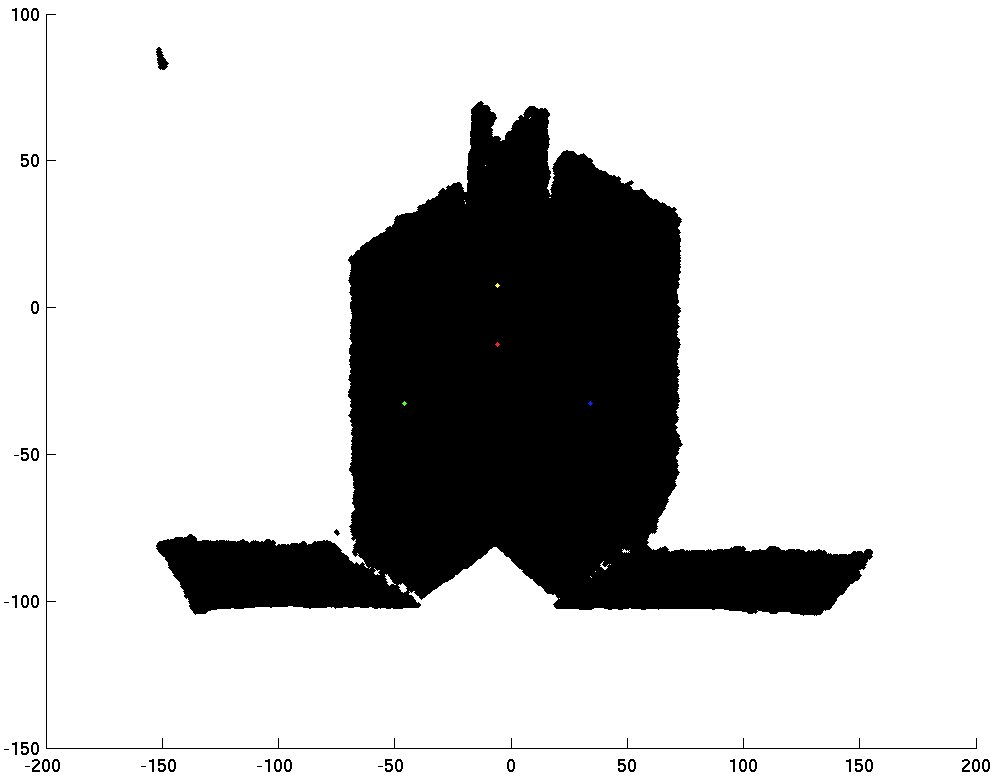
\includegraphics[width=\textwidth]{Images/4-Points(1).png}
		\caption{}
		\label{fig:points}
	\end{subfigure}%
	\hspace{1cm}
	\begin{subfigure}[b]{0.45\textwidth}
		\centering
		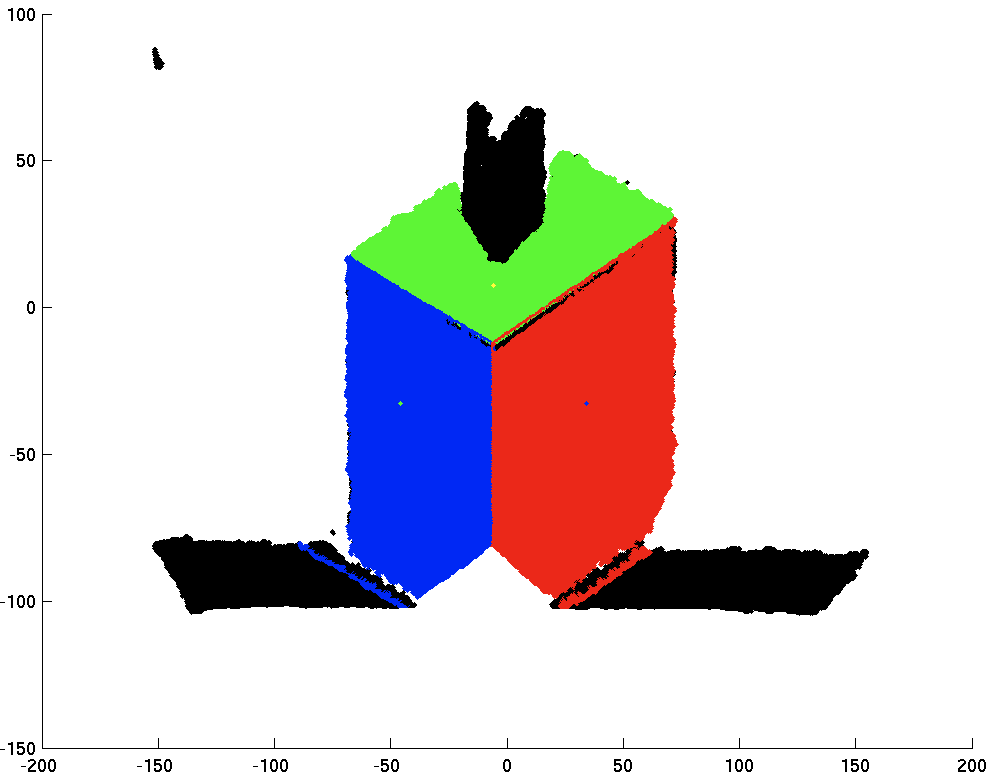
\includegraphics[width=\textwidth]{Images/5-RegionGrowing(1).png}
		\caption{}
		\label{fig:regionGrowing}
	\end{subfigure}
	\caption{Reduced point cloud data with the corner point (red) and the three approximation points for the three planes (a) and region growing with initialization on the closest patch to the points (b).}
\end{figure}

\subsubsection{Region Growing}
In our region growing algorithm we used a plane tolerance of 1 and point distance tolerance of 150. By having a low plane tolerance we acquired more accurate regions and with such a large point distance tolerance the growing only needed about 5 iterations. When the number of new points in a region exceeded the number of points already in the region plus 50 then a plane is (re)fitted to the region. The region growing stops when the least square fitting error of that plane is bigger than 30\% of the number of new points.


